Les différents services proposés du côté du personnel de la maintenance sont illustrés sur la figure \ref{maintenance}.
\newline
\begin{figure}[h!]
	\hspace*{-2.5cm}
	\centering
	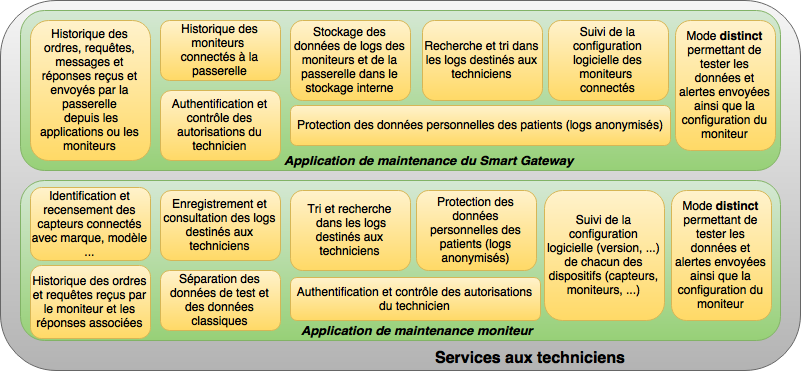
\includegraphics[width=1.4\textwidth]{maintenance.png}
	\caption{Services de la Couche Applicative du côté du Personnel de la Maintenance}
	\label{maintenance}
\end{figure}

Un hôpital doit avoir un équipement le plus fiable possible. En effet, une simple défaillance peut causer la mort du patient, ou
à défaut de graves dommages. Il est donc important de choisir prudemment les équipements à utiliser. Malheureusement l'équipement
sans faille n'existe pas et lorsqu'une panne se produit, il est capital de pouvoir déterminer l'origine de la défaillance. Pour
cela la présence de logs est indispensable à tous les niveaux. 
\newline

Au niveau du moniteur, il faut pouvoir savoir quel type de capteur s'est connecté (marque, modèle) afin d'identifier d'éventuelles
incompatibilités. Il faut également enregistrer les moments où le moniteur a donné un ordre, ainsi que son contenu.
Les réponses reçues sont aussi à conserver.
\newline

La passerelle intelligente (parfois appelée smart gateway) doit également avoir un historique des messages/demandes qu'elle a
reçus. Allié avec les logs issus d'un moniteur cela peut permettre d'identifier des problèmes réseaux, des interblocages et bien
d'autres dysfonctionnements.
\newline 

Pour des raisons similaires, des logs doivent être aussi présents au niveau du stockage interne et du cloud. En plus de permettre
une meilleure compréhension des pannes, ils pourraient avoir des applications au niveau de la sécurité. Entre autre, ils seraient
un moyen simple pour s'assurer que personne n'a essayé d'accéder à données qui ne leur sont pas destinées.
\newline

La présence de logs, impose de pouvoir les gérer. En effet, ces logs risquent d'être volumineux, il faut donc avoir la
possibilité de trier ces derniers afin de ne récupérer que les données pertinentes. Mettons que l'on ait l'intégralité des logs
d'une passerelle intelligente, il serait souhaitable de pouvoir extraire toutes les données relatives à un moniteur. De ce fait,
il faut intégrer un module de récupération de données permettant de filtrer les données via une description de ce que l'on veut
récupérer. Idéalement et afin d'être le plus flexible possible, ces descriptions seraient faites via un langage de requêtes
structurées. En effet, les données et capteurs utilisés peuvent varier d'un patient à l'autre, aussi lors de l'enquête suite à une
panne ou lors de tests, il est important faire du cas par cas et ne pas être prisonnier d'outils trop généraux.
\newline

Par ailleurs, la récupération de ses logs doit se faire de manière distincte de l'obtention des données d'un patient. Ces logs
étant destinés au service technique, aucune information personnelle ne doit transparaître. En particulier, ni le nom ni l'id du
patient ne doivent être visibles. De plus, le service technique doit savoir quelle version de chaque logiciel est présent sur
chaque objet connecté de l'hôpital. Cela permettrait d'agir efficacement si un bug, problème de compatibilité, etc ... Venait à se
produire.
\newline

Enfin, le système doit avoir un module consacré aux tests. Les équipements (moniteurs, passerelles) ont un rôle capital et une
défaillance de leur part aurait de graves conséquences. Aussi, le système doit faciliter la conception et mise en place de tests.
Pour cela, notre plateforme doit comporter un mode \textit{test} qui permettrait au technicien de suivre les données qu'il envoie.
Ce mécanisme permettrait la vérification de l'acheminement des données et que des décisions appropriées sont prises au regard de
ces dernières. Ce mode devra également permettre plus de contrôle: si une donnée de test relative à un taux de glucose trop élevé
est envoyée, il ne faut pas que le personnel médical soit dérangé car il s'agit de données fictives. Mais afin de vérifier
l'émission d'alerte, il est préférable que le technicien puisse préciser où l'alerte sera envoyée (probablement sur l'une des
machines dédiées aux tests que le service technique a en sa possession). Un autre requis de ce système est une dissociation entre
le mode test (ses données, ses décisions) et le fonctionnement du mode normal. Ces deux modes vont sûrement se côtoyer, mais il
est impensable que l'un interfère avec l'autre. Si les données venaient à se mélanger, cela pourrait être dangereux pour le
patient : un médecin pourrait prendre des décision basées sur des données fictives (destinées aux tests). De plus, si le service
technique venait à avoir accès à des données d'un patient (suit à un mélange entre les deux types de données), cela
représenterait une atteinte à la vie privée. Et il faut garantir que les réglages faits pour les tests ne se propage pas en dehors
du domaine de test, sinon le bien être et la santé des patients est à risque.
\newline

Dans le but de lever toute ambigüité, nous allons maintenant détailler les requis qu'un système de ce type devrait supporter.
\begin{enumerate}
    \item disponibilité et fiabilité: si un problème survient, il faut pour le diagnostiquer rapidement. Pour cela il faut que le
    système soit accessible et que, si une panne venait à se produire, cette dernière n'entrave pas le bon fonctionnement. Ou du
    moins pendant un temps raisonnable.
    \item authentification: afin de préserver la sécurité, il est souhaitable que seul le service de maintenance ait accès à ce
    service. La présence d'un mécanisme d'authentification est donc nécessaire.
    \item anonymiser: les logs ne doivent pas permettre d'identifier le patient auxquels ils se rapportent. Il est possible que
    certaines situations exigent de connaître plus de données afin d'identifier un dysfonctionnement. L'obtention de ces données
    devra se faire par le bais d'un médecin.
    \item gestion et contrôle des ressources: connaître l'identité de chaque dispositif (marque/modèle) faciliterait le travail de
    maintenance.
\end{enumerate}
